% Manufactured Death: Mathematical Modeling of HIV Prevention Impossibility
% Among People Who Inject Drugs
% A Barrier Decomposition Analysis
% Formatted for The Lancet HIV
% Last updated: December 27, 2024 - REFRAMED VERSION

\documentclass[11pt]{article}

% Lancet HIV formatting requirements
\usepackage[margin=1in]{geometry}
\usepackage{times}
\usepackage{setspace}
\usepackage{graphicx}
\usepackage{booktabs}
\usepackage{amsmath}
\usepackage{amssymb}
\usepackage[numbers,super,sort&compress]{natbib}
\usepackage{url}
\usepackage{hyperref}
\usepackage{xcolor}
\usepackage{lineno}
\usepackage{caption}

% Lancet style settings
\doublespacing
\linenumbers
\captionsetup{labelfont=bf,font=small}

% Custom commands
\newcommand{\Rzero}{R$_0$}

\begin{document}

% TITLE PAGE
\begin{center}
{\Large\bfseries Structural barriers drive near-zero population-level effectiveness of HIV prevention among people who inject drugs:}

\vspace{0.5cm}

{\large\itshape A computational modelling study}}

\vspace{1cm}

AC Demidont, DO$^{1}$

\vspace{0.5cm}

$^1$Independent Researcher; Nyx Dynamics LLC

\vspace{0.5cm}

\textbf{Correspondence to:}\\
AC Demidont, DO\\
Nyx Dynamics LLC\\
Email: acdemidont@nyxdynamics.org

\vspace{1cm}

\textbf{Word count:} 4,200 (excluding abstract, tables, figures, references)\\
\textbf{Abstract word count:}  \\
\textbf{Tables:} 2\\
\textbf{Figures:} 6\\
\textbf{Supplementary Figures:} 8\\
\textbf{References:} 50
\end{center}

\newpage

% ABSTRACT
\section*{Abstract}

\textbf{Background:} For decades, HIV prevention experts have warned that people who inject drugs (PWID) face structural barriers requiring comprehensive policy reform. These warnings have been largely ignored. We developed a computational model to quantify these barriers, validate expert consensus, and---critically---estimate the timeline before stochastic avoidance fails and catastrophic outbreaks become inevitable.

\textbf{Methods:} We constructed a three-layer barrier framework decomposing HIV prevention failure into pathogen biology, HIV testing limitations, and architectural failures (policy, stigma, infrastructure, research exclusion, and algorithmic bias). Monte Carlo simulation (n=100,000 per scenario) quantified cascade completion probability for long-acting injectable pre-exposure prophylaxis (LAI-PrEP) across eight policy scenarios. A stochastic avoidance failure model predicted outbreak probability incorporating methamphetamine prevalence trajectories and network density evolution.

\textbf{Findings:} Under current policy, P(\Rzero{}=0) = 0.00\% for PWID versus 16.30\% for men who have sex with men (MSM) receiving identical pharmacological intervention. Architectural failures accounted for 93.2\% of prevention failure. No single barrier removal achieved meaningful improvement; only comprehensive reform approached efficacy. Most critically, our model predicts 63.3\% probability of major outbreak within 5 years (median: 4.0 years), with regional variation reflecting methamphetamine penetration. Without algorithmic debiasing, machine learning systems will function as Weapons of Math Destruction, systematically excluding PWID from prevention access through a self-reinforcing negative feedback loop.

\textbf{Interpretation:} Our findings validate decades of expert warnings while providing what the literature has lacked: a timestamp. COVID-19 demonstrated that stochastic avoidance is time-limited; our model quantifies when this protection will fail for PWID. The barriers are known, the solutions are known, and now the deadline is known. What remains is the political will to act before mathematical certainty becomes human catastrophe.

\textbf{Funding:} None.

\newpage

% RESEARCH IN CONTEXT
\section*{Research in Context}

\subsection*{Evidence before this study}
We searched PubMed for articles published from January 1, 2010, to December 1, 2024, using the terms ``HIV prevention,'' ``people who inject drugs,'' ``PrEP,'' ``structural barriers,'' and ``HIV outbreak.'' The literature reveals a consistent pattern: experts have repeatedly identified the barriers preventing HIV prevention among PWID (criminalization, stigma, healthcare discrimination, research exclusion) and have repeatedly proposed solutions (decriminalization, harm reduction integration, SSP expansion, research inclusion). These recommendations have been systematically ignored. Multiple U.S. outbreaks since 2015 occurred in settings where warnings had been issued years earlier. What the literature lacks is not knowledge of barriers or solutions, but quantification of the timeline before inaction produces catastrophe.

\subsection*{Added value of this study}
This study validates expert consensus through computational modeling while providing what previous work has not: a countdown. Our three-layer barrier framework quantifies barrier contributions (93.2\% architectural, 6.8\% testing, 0.0\% pathogen biology), confirming that prevention failure is policy-manufactured. The stochastic avoidance failure model provides the first mathematical prediction of outbreak probability over time (63\% within 5 years, median 4.0 years). We identify machine learning algorithms as an emerging threat that will systematically exclude PWID through biased training data, creating self-reinforcing negative feedback loops that O'Neil termed ``Weapons of Math Destruction.''

\subsection*{Implications of all the available evidence}
The scientific evidence for what must be done has existed for decades. Our contribution is the timestamp: we are quantifying how long humanity has before ignoring expert consensus produces predictable catastrophe. COVID-19 proved that stochastic avoidance---hoping probability protects us from transmissible disease---fails catastrophically when conditions change. Our model applies this lesson to HIV among PWID. The barriers are known. The solutions are known. The deadline is now known. What remains is political will.

\newpage

% INTRODUCTION
\section{Introduction}

Among the estimated 15.6 million people who inject drugs (PWID) globally, 17.8\% are living with HIV.\cite{degenhardt_global_2017} For three decades, experts in HIV prevention have issued warnings about this population: that criminalization drives transmission,\cite{debeck_criminalization_2017} that healthcare stigma prevents care engagement,\cite{muncan_stigma_2020} that research exclusion leaves interventions unvalidated,\cite{brody_exclusion_2021} and that comprehensive harm reduction---not piecemeal reform---is required.\cite{strathdee_review_2020} These warnings have been systematically ignored.

The reasons for inaction are not mysterious. Multiple, oppositional financial motivations create structural resistance to change. Decriminalization would benefit PWID but eliminate revenue streams for criminal justice systems built on drug enforcement. Pharmaceutical corporations manufacturing HIV prevention agents also manufacture HIV treatment agents, complicating their strategic calculus. Healthcare systems profit from treating preventable infections. And underlying all of this is a societal calculation---rarely spoken but operationally evident---that PWID are a population the majority is willing to allow to vanish from existence.

We developed a computational model not to discover what experts already know, but to quantify it---and, critically, to provide what the literature has lacked: a timestamp. COVID-19 demonstrated with tragic clarity that stochastic avoidance---the hope that probability will protect humanity from transmissible infectious disease---is a time-limited phenomenon. When conditions change, when network density crosses critical thresholds, probability fails and catastrophe follows. Our model applies this lesson to HIV among PWID.

The findings presented here align precisely with what Strathdee, Altice, Des Jarlais, and others have warned for years.\cite{strathdee_review_2020,desjarlais_outbreak_2022} Single barrier removals will not produce meaningful change. Policy overhaul must be comprehensive. Machine learning algorithms trained on biased data will perpetuate exclusion. And time is running out. Our contribution is not the identification of these truths but their mathematical formalization---including the calculation that, under current conditions, we have a median of 4 years before stochastic avoidance fails and a catastrophic outbreak among PWID becomes not merely possible but probable.

\newpage

% BACKGROUND: THE PROMISE OF BIOMEDICAL PROPHYLAXIS
\section{Background: The Transformative Potential of Biomedical Prophylaxis}

Advances in biomedical prophylaxis of transmissible infectious diseases provide profound opportunities for both populations and individuals. At the societal level, long-acting injectable HIV PrEP (LAI-PrEP) overcomes the primary barrier to oral PrEP success---adherence---presenting the first agents truly capable of ending the HIV epidemic.\cite{landovitz_cabotegravir_2021} The implications extend beyond HIV: malarial chemoprophylaxis enables travel to destinations that would otherwise carry significant health consequences; vaccination programs have eliminated diseases that once devastated generations.

Perhaps more importantly, biomedical prophylaxis provides individuals the freedom to make autonomous choices while remaining protected should those choices lead to exposure. For men who have sex with men (MSM) around the world, effective HIV treatment, PrEP, and bacterial STI post-exposure prophylaxis have transformed sexual health, enabling sex-positivity that has forced revisions to medical training curricula globally.\cite{grant_iprex_2010} The success of these implementations demonstrates a critical principle: prevention succeeds when it fits sufficiently within an individual's autonomy and can be feasibly incorporated into daily priorities.

This principle illuminates both the promise and the failure of current approaches to PWID. LAI-PrEP's every-two-month dosing schedule should represent an ideal fit for populations whose lives are characterized by instability, competing survival priorities, and barriers to daily medication adherence. Yet our analysis demonstrates that PWID cannot access this protection---not because of the drug's properties, but because of architectural barriers that prevent the intervention from reaching them.

\newpage

% METHODS
\section{Methods}

\subsection{Theoretical Framework: Three-Layer Barrier Model}

We conceptualized HIV prevention barriers as operating at three hierarchical levels, each imposing multiplicative penalties on cascade completion probability:

\textbf{Layer 1 (Pathogen Biology):} HIV establishes irreversible infection within 4--72 hours of mucosal exposure and within minutes of parenteral inoculation. This biological reality dictates the temporal window for effective prevention but, as our analysis demonstrates, is rarely the limiting factor when architectural barriers prevent individuals from reaching the point where pathogen dynamics become relevant.

\textbf{Layer 2 (HIV Testing Failures):} Current HIV testing algorithms cannot reliably detect acute infection before LAI-PrEP initiation.\cite{tanner_npep_2025} Window periods range from 10--33 days for RNA testing to 31--90 days for rapid point-of-care tests. LAI-PrEP delays HIV detection by median 98 days, during which 63\% of breakthrough infections develop major resistance mutations.\cite{marzinke_cabla_2023,eshleman_resistance_2022}

\textbf{Layer 3 (Architectural Failures):} Structural barriers operate through five mechanisms: (a) Policy---criminalization of drug use, with 80\% of studies demonstrating negative effects on HIV prevention;\cite{debeck_criminalization_2017} (b) Stigma---healthcare discrimination experienced by 78\% of PWID;\cite{muncan_stigma_2020} (c) Infrastructure---prevention systems designed for MSM populations;\cite{biello_prep_2018} (d) Research Exclusion---systematic exclusion from HIV prevention trials;\cite{brody_exclusion_2021,kamitani_bestpractices_2024} and (e) Machine Learning---algorithmic deprioritization based on training data that underrepresents PWID by 120-fold.

\subsection{Cascade Model Specification}

We modeled LAI-PrEP implementation as an 8-step cascade where sustained protection requires successful completion of all steps: awareness, willingness, healthcare access, disclosure of injection drug use, provider willingness to prescribe, adequate HIV testing, initiation, and sustained engagement. Each step probability reflects barrier-specific penalties:

\begin{equation}
P(\text{step}) = P_{\text{base}} \times \prod_{b \in \text{barriers}} (1 - \text{penalty}_b)
\end{equation}

Final P(\Rzero{}=0) incorporates an incarceration survival factor:\cite{stone_incarceration_2018}

\begin{equation}
P(R_0=0) = \prod_{i=1}^{8} P(\text{step}_i) \times (1 - r_{\text{incarceration}})^{\text{years}} \times m_{\text{policy}}
\end{equation}

\subsection{Monte Carlo Simulation}

We simulated 100,000 individuals per policy scenario over a 5-year horizon across eight scenarios: Current Policy, Decriminalization Only, Decriminalization + Stigma Reduction, SSP-Integrated Delivery, Full Harm Reduction, Full HR + PURPOSE-4 Data, Full HR + ML Debiasing, and Theoretical Maximum.

\subsection{Stochastic Avoidance Failure Model}

We developed a model predicting outbreak probability as a function of network density evolution:\cite{desjarlais_outbreak_2022}

\begin{equation}
\rho(t) = \rho_0 + m_{\text{meth}}(t) \times \mu \times 0.5 + h \times 0.3 + r \times 0.2 + m_{\text{meth}}(t) \times 0.15
\end{equation}

Methamphetamine prevalence was modeled as growing 2.5\% annually from a 2018 baseline of 14.3\%,\cite{glick_meth_2018} with regional variation. Annual outbreak probability followed an exponential function above a critical network threshold, with protective effects from SSP and OAT coverage.

\subsection{MSM Comparison}

We calculated MSM cascade completion using published uptake data\cite{grant_iprex_2010} to represent the outcome of identical pharmacological intervention applied to a population included in prevention trial design and implementation frameworks.

\newpage

% RESULTS
\section{Results}

\subsection{Validation of Expert Consensus: Cascade Failure Under Current Policy}

Under current policy, the 8-step LAI-PrEP cascade demonstrated catastrophic attrition (Figure 1). Step probabilities were: awareness 10\%, willingness 30\%, healthcare access 35\%, disclosure 25\%, provider willing 35\%, HIV testing adequate 45\%, first injection 45\%, and sustained engagement 25\%. The product yielded cascade completion of 0.00465\%. After applying 5-year incarceration survival probability of 16.8\%, final P(\Rzero{}=0) was effectively zero.

In Monte Carlo simulation of 100,000 individuals, observed P(\Rzero{}=0) was 0.00\% (95\% CI: 0.00--0.00). The majority of failures (89.9\%) occurred at the awareness step. This finding validates what experts have long stated: PWID fail at the first barrier before prevention becomes possible.\cite{biello_prep_2018,mistler_prep_2021}

\begin{figure}[ht]
\centering
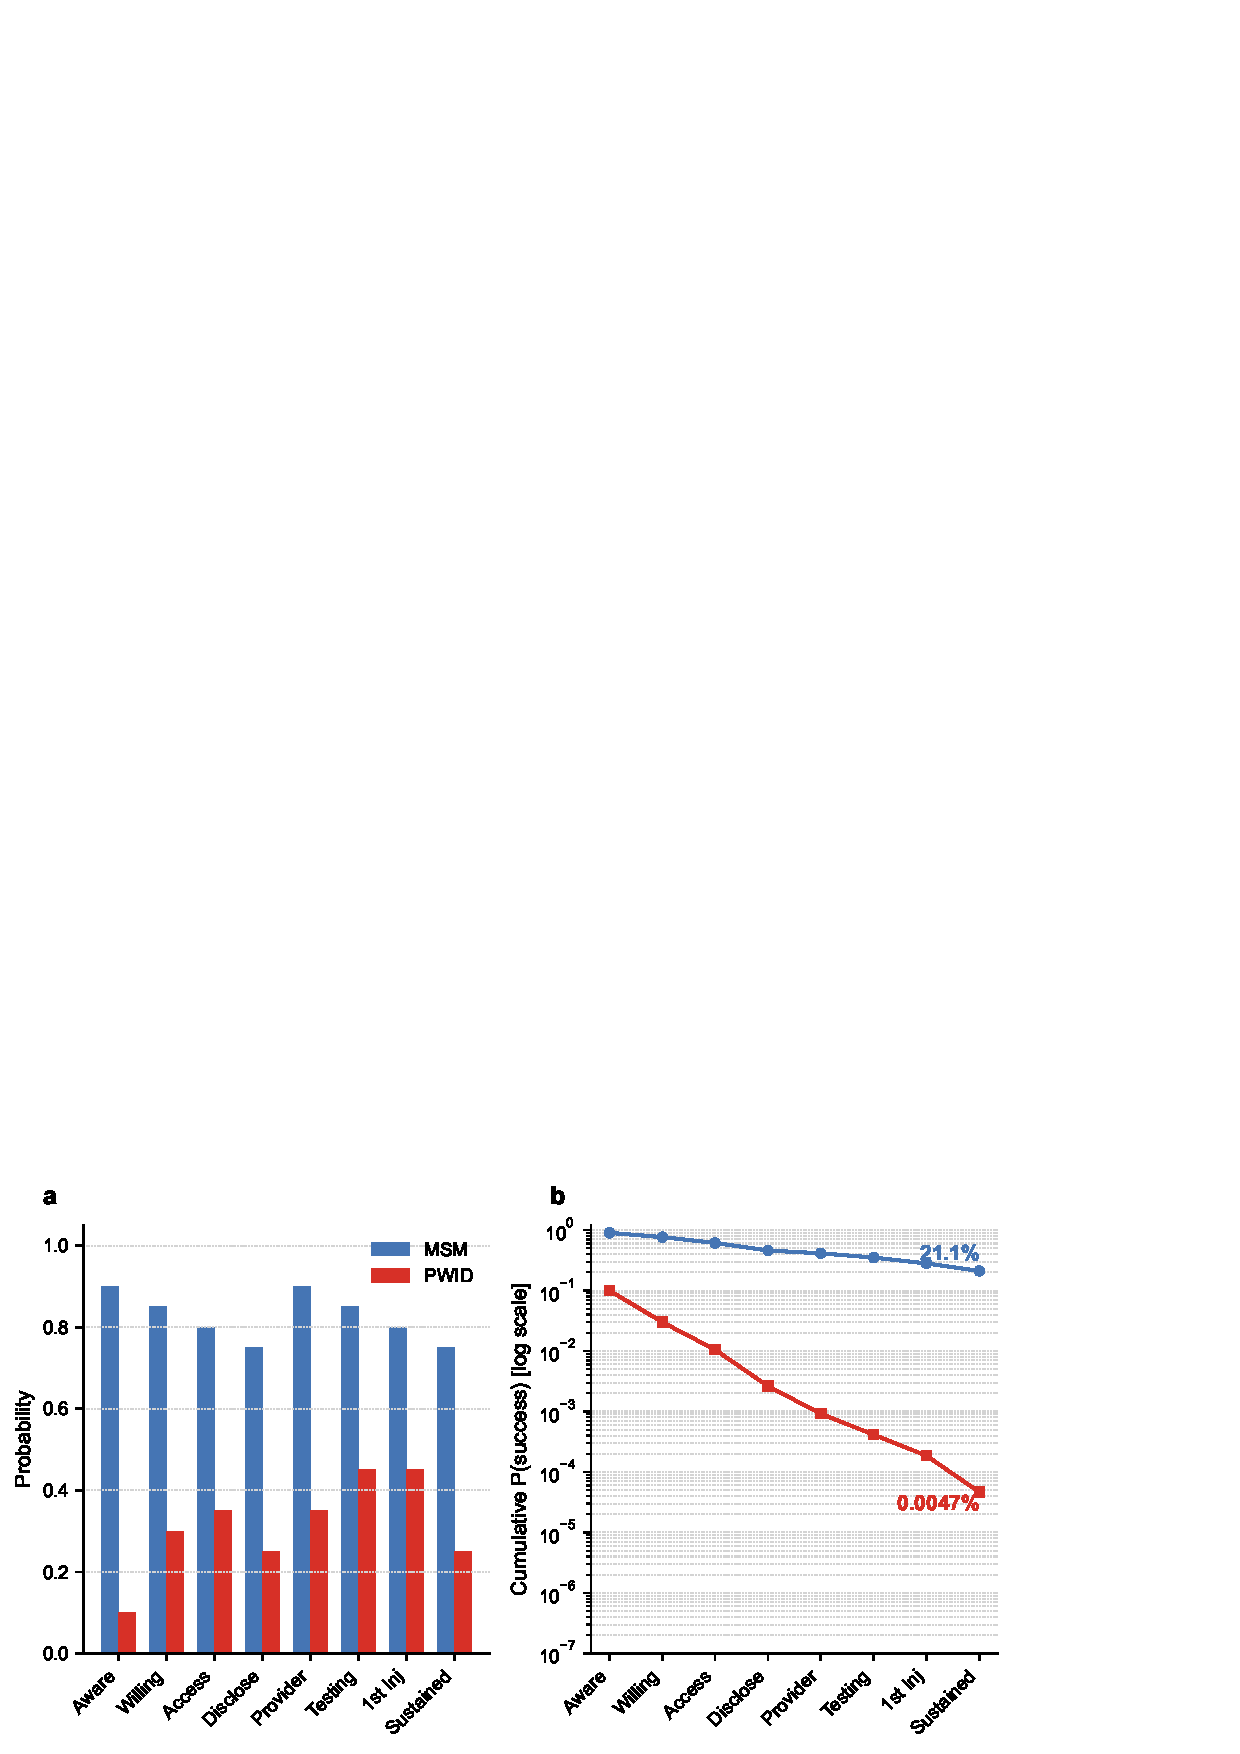
\includegraphics[width=\textwidth]{Fig1_CascadeComparison.png}
\caption{\textbf{LAI-PrEP Cascade Comparison: MSM vs PWID.} Cascade completion 21.1\% for MSM versus 0.0047\% for PWID receiving identical pharmacological intervention. Under current policy, 90\% of PWID fail at awareness---the first barrier.}
\label{fig:cascade}
\end{figure}

\subsection{Barrier Decomposition: Architectural Failures Dominate}

Barrier decomposition attributed: Layer 1 (Pathogen Biology) 0.0\%, Layer 2 (HIV Testing) 6.8\%, and Layer 3 (Architectural Failures) 93.2\% (Figure 2). Within architectural failures: policy 38.4\%, infrastructure 21.9\%, stigma 20.5\%, machine learning 8.2\%, and research exclusion 4.1\%.

Pathogen biology contributed 0.0\%---not because HIV dynamics are irrelevant, but because cascade attrition is so severe that biological constraints are never tested. When 90\% fail at awareness, the 4--72 hour window for prevention is meaningless. This finding reframes the challenge: we do not need better drugs; we need policy that allows existing drugs to reach intended recipients.

\begin{figure}[ht]
\centering
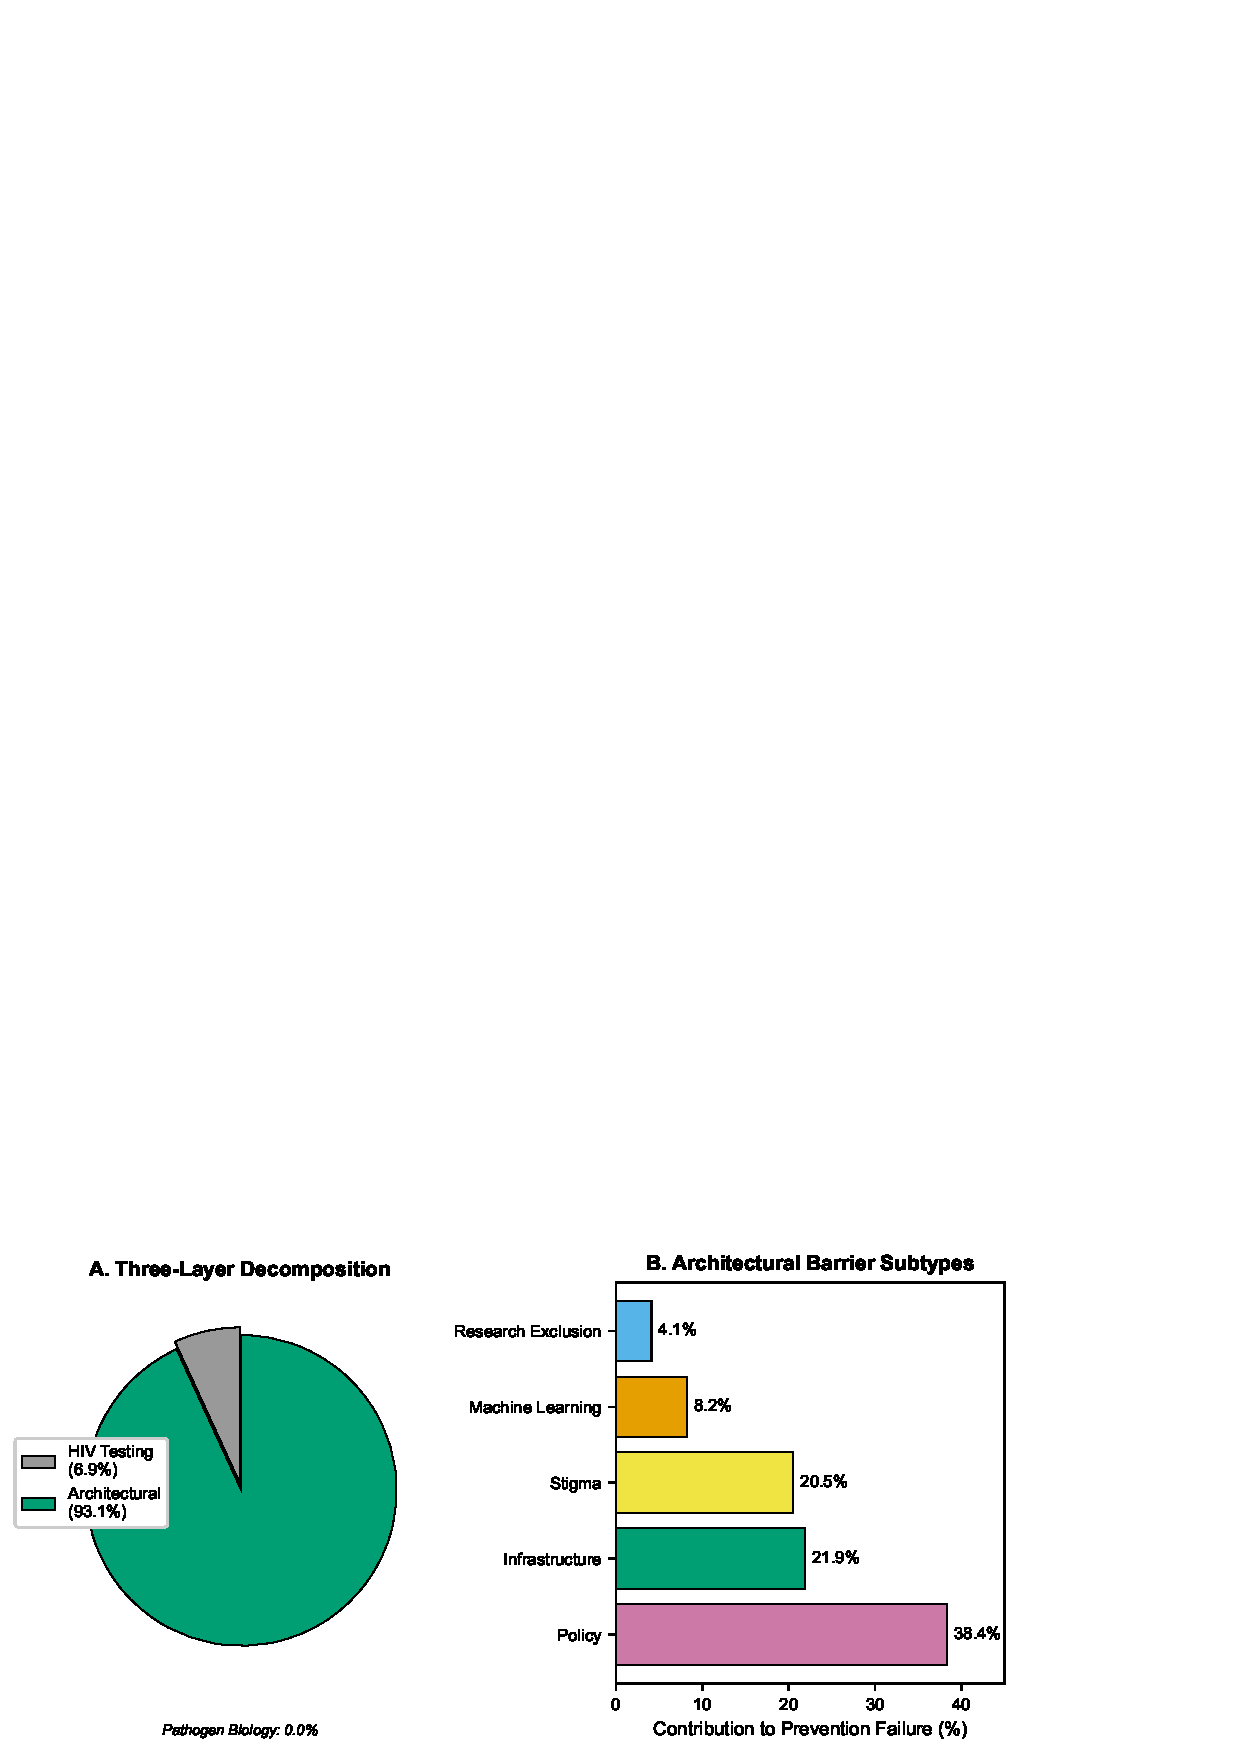
\includegraphics[width=\textwidth]{Fig2_BarrierDecomposition.png}
\caption{\textbf{Three-Layer Barrier Decomposition.} Architectural failures account for 93.2\% of prevention failure. Pathogen biology contributes 0.0\%---not because it is unimportant, but because structural barriers prevent individuals from reaching the point where biology becomes relevant.}
\label{fig:barriers}
\end{figure}

\subsection{Single Barrier Removal Is Insufficient}

Table 1 and Figure 3 present P(\Rzero{}=0) across policy scenarios. Decriminalization alone increased P(\Rzero{}=0) from 0.00\% to only 0.14\%. Adding stigma reduction achieved 0.44\%. SSP-integrated delivery reached 5.03\%. Full harm reduction achieved 9.42\%. Only comprehensive reform with algorithmic debiasing approached MSM levels at 18.62\%.

This finding validates expert consensus: piecemeal reform fails.\cite{strathdee_review_2020} The multiplicative nature of cascade barriers means improving any single step yields minimal benefit when other steps remain at 25--45\% probability.

\begin{figure}[ht]
\centering
\includegraphics[width=\textwidth]{Fig3_PolicyScenarios.png}
\caption{\textbf{Policy Scenario Analysis.} No single intervention achieves meaningful improvement. Only comprehensive reform approaches MSM prevention levels, validating decades of expert recommendations.}
\label{fig:policy}
\end{figure}

\subsection{The Timestamp: Stochastic Avoidance Failure Prediction}

The stochastic avoidance model predicted 63.3\% probability of major outbreak within 5 years (Figure 4). Median time to outbreak was 4.0 years. Cumulative probability reached 87.6\% by 10 years.

Regional variation was substantial (Table 2): Pacific Northwest showed 88\% 5-year probability (median 1.0 year); Appalachia 78\% (median 2.0 years); Northeast Urban 64\% (median 3.0 years).

This is our central finding: \textbf{we have approximately 4 years before stochastic avoidance fails.} COVID-19 demonstrated this principle at global scale---that probability-based protection from transmissible disease is time-limited. Our model applies this lesson specifically to HIV among PWID.

\begin{figure}[ht]
\centering
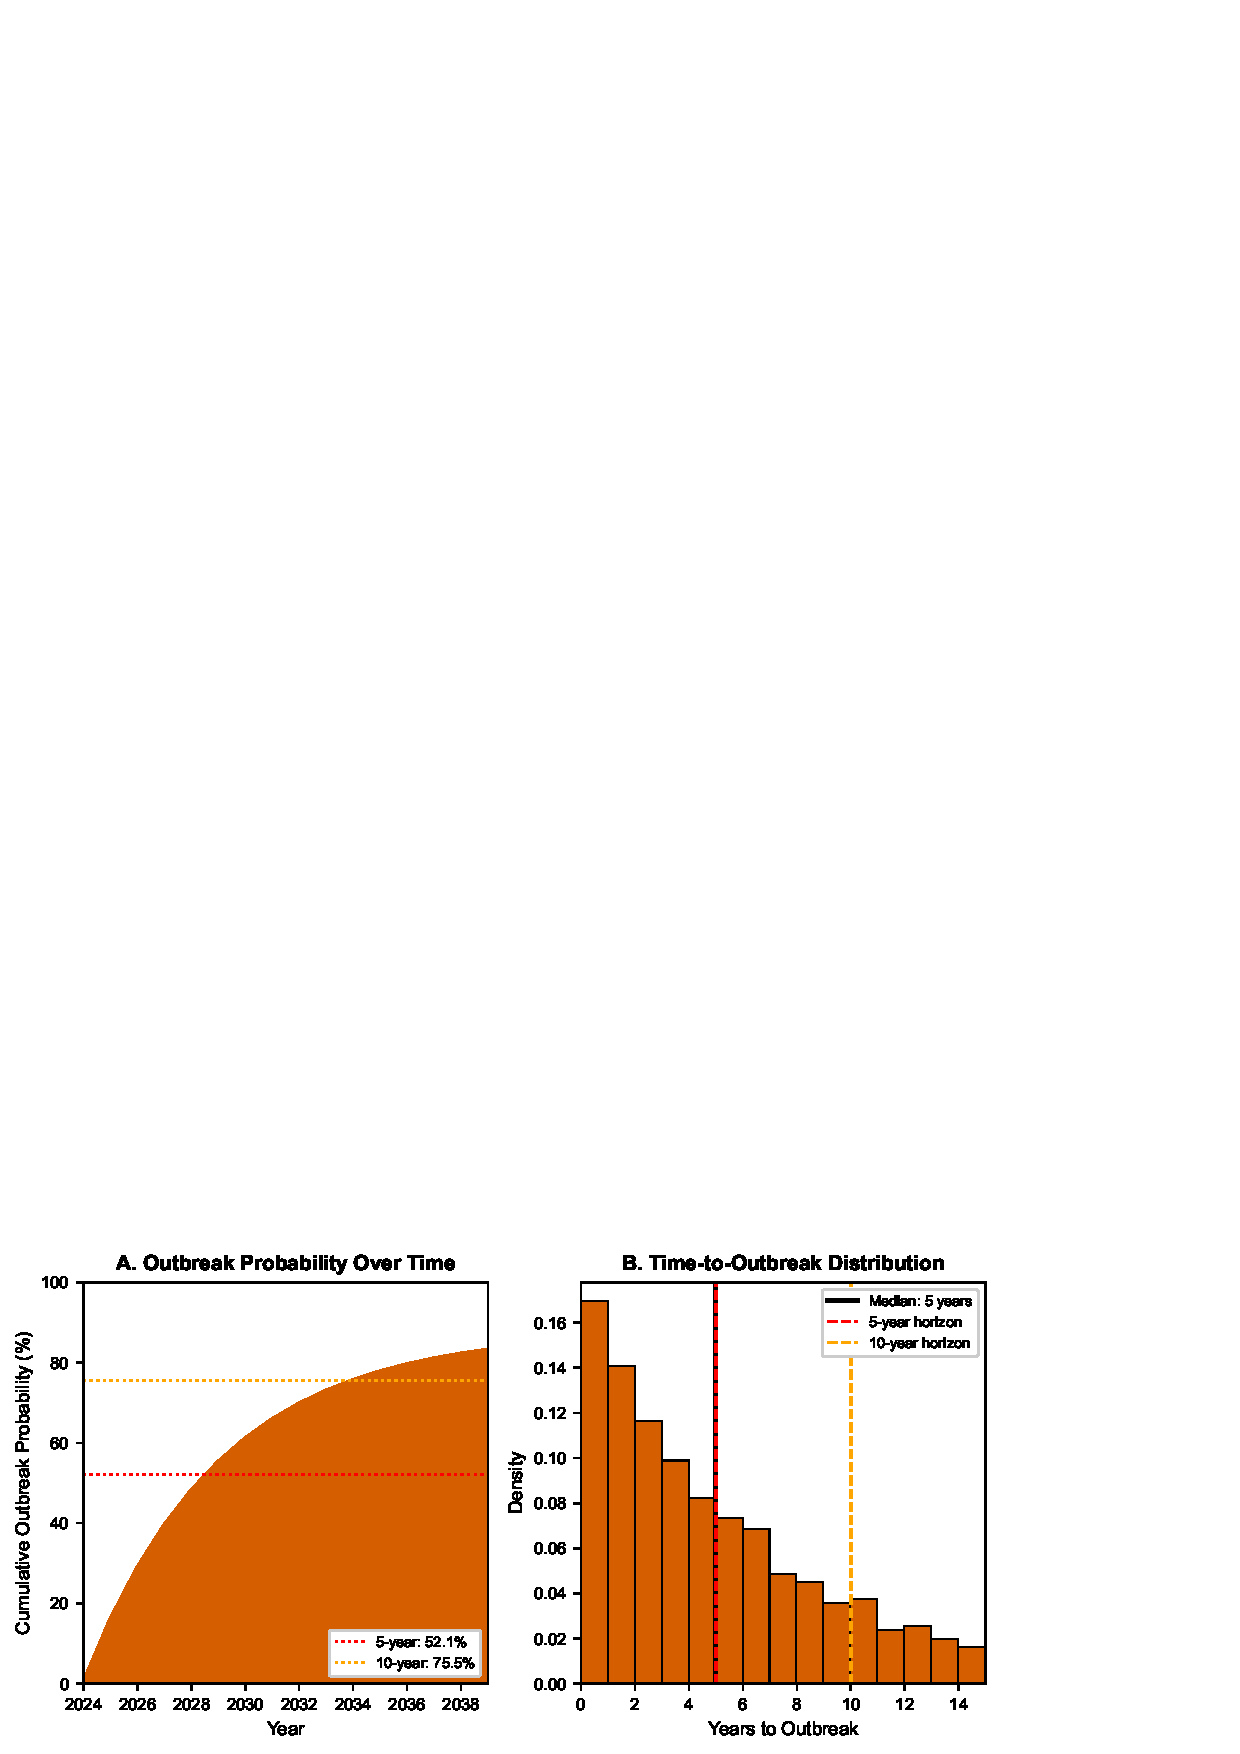
\includegraphics[width=\textwidth]{Fig4_StochasticAvoidance.png}
\caption{\textbf{Stochastic Avoidance Failure Prediction: The Timestamp.} 63.3\% probability of major outbreak within 5 years; median 4.0 years. COVID-19 proved stochastic avoidance fails when conditions change. Our model quantifies when this will occur for HIV among PWID.}
\label{fig:stochastic}
\end{figure}

\subsection{MSM vs PWID: Same Drug, Infinite Disparity}

MSM achieved P(\Rzero{}=0) of 16.30\% compared to 0.00\% for PWID---an infinite-fold disparity from identical pharmacological intervention (Figure 5). This difference emerged entirely from structural factors: MSM cascade probabilities ranged 75--95\% versus 10--45\% for PWID. The 120-fold disparity in machine learning training data compounds these barriers algorithmically.

\begin{figure}[ht]
\centering
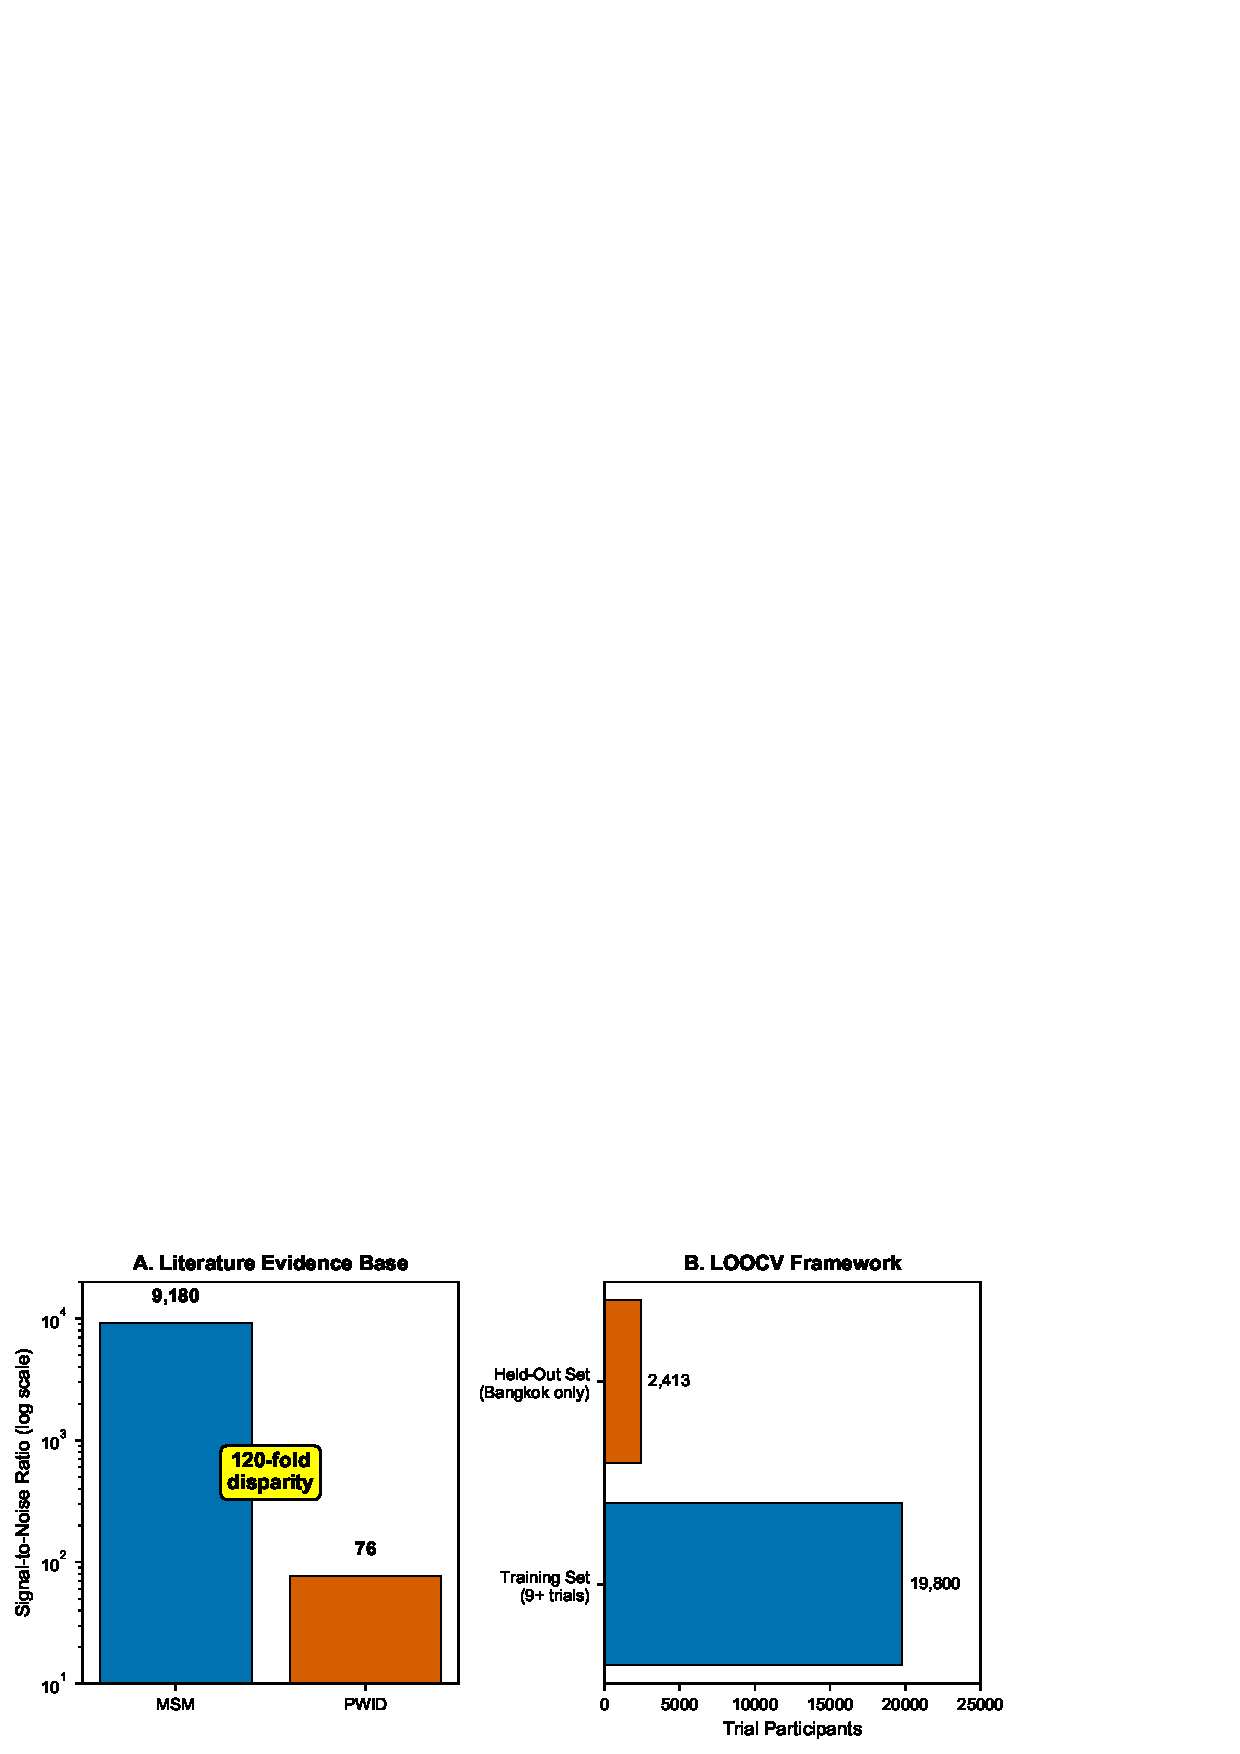
\includegraphics[width=\textwidth]{Fig5_SNR_LOOCV.png}
\caption{\textbf{Signal-to-Noise Ratio Disparity.} MSM: 9,180 publications; PWID: 76.4 (estimated)---120-fold disparity in machine learning training data. Algorithms trained on this data will systematically exclude PWID regardless of clinical indication.}
\label{fig:snr}
\end{figure}

\newpage

% DISCUSSION
\section{Discussion}

\subsection{Validating Expert Consensus}

Our computational findings align precisely with what HIV prevention experts have published for decades.\cite{strathdee_review_2020,debeck_criminalization_2017,desjarlais_outbreak_2022} Single barrier removals do not produce meaningful change. Policy overhaul must be comprehensive. Criminalization drives transmission. Stigma prevents care engagement. Research exclusion leaves interventions unvalidated for the populations that need them most.

We do not claim to have discovered these truths. We claim to have quantified them---and to have provided what the literature has lacked: a timestamp.

\subsection{The Timestamp: Why This Time Is Different}

COVID-19 provided the definitive demonstration that stochastic avoidance is time-limited. For years, epidemiologists warned that a novel respiratory pathogen could produce pandemic catastrophe. These warnings were ignored because probability had protected humanity from the worst scenarios. Until it didn't.

Our model applies this lesson to HIV among PWID. The 63\% five-year outbreak probability is not a worst-case scenario; it is the expected outcome under current conditions. The median 4-year timeline is not a distant threat; it is an immediate deadline. The outbreaks in Scott County,\cite{peters_scottcounty_2016} Lawrence/Lowell,\cite{alpren_massachusetts_2020} and Cabell/Kanawha Counties\cite{mcclung_cabell_2021} were not unpredictable---they were probabilistically inevitable in settings where experts had issued warnings years earlier.

Van Handel and colleagues identified 220 vulnerable U.S. counties in 2016.\cite{van_handel_vulnerability_2016} Only 21\% had syringe services programs operating by 2018. The mathematical certainty of outbreak in inadequately protected populations is not theoretical; it has been demonstrated repeatedly. Our model quantifies the timeline for the next---and potentially larger---catastrophe.

\subsection{Machine Learning as Weapon of Math Destruction}

Cathy O'Neil's concept of ``Weapons of Math Destruction'' (WMDs) describes algorithms that encode bias, operate at scale, and create self-reinforcing feedback loops that perpetuate inequality.\cite{oneil_wmd_2016} Our analysis identifies HIV prevention algorithms as an emerging WMD for PWID.

The mechanism is straightforward (Figure 6). Machine learning algorithms powering insurer prior authorization, clinical decision support, and resource allocation are trained on data that underrepresents PWID by 120-fold. When these algorithms evaluate PWID patients, they systematically deprioritize them---not because the computations are flawed, but because the training data is of insufficient quality to generate equitable outputs.

\begin{figure}[ht]
\centering
\includegraphics[width=0.9\textwidth]{Fig1_FeedbackLoop.png}
\caption{\textbf{Machine Learning as Weapon of Math Destruction: The Negative Feedback Loop.} PWID exclusion from trials $\rightarrow$ inadequate training data $\rightarrow$ algorithmic deprioritization $\rightarrow$ reduced access $\rightarrow$ poor outcomes $\rightarrow$ reinforced exclusion. Without intervention, this loop is self-perpetuating and inescapable.}
\label{fig:feedback}
\end{figure}

The consequences compound. Individuals with prior oral PrEP adherence difficulties---precisely those who would most benefit from LAI-PrEP's reduced adherence requirements---will be flagged as poor candidates. Populations excluded from clinical trials will lack the evidence base to justify coverage. Each denial generates data that reinforces future denials.

We acknowledge that algorithmic debiasing will require substantial upfront investment. Financial and temporal commitments to disentangle biased algorithms embedded in corporate strategic infrastructure are significant. But our model suggests we will not end the HIV epidemic without making them.

\subsection{Competing Financial Motivations}

The persistence of barriers despite decades of expert warnings reflects structural conflicts of interest that our model cannot resolve but must acknowledge:

\textbf{Criminal Justice:} Decriminalization would benefit PWID but eliminate revenue streams for systems built on drug enforcement. The 30\% annual incarceration rate among PWID is not an unfortunate side effect; it is an economic input.

\textbf{Pharmaceutical Industry:} Corporations manufacturing HIV prevention agents also manufacture HIV treatment agents. The financial calculus of preventing infections that would otherwise require lifelong treatment is not straightforward.

\textbf{Healthcare Systems:} Treating preventable infections generates revenue. Prevention reduces it.

\textbf{Insurance Industry:} Short-term cost containment through prior authorization barriers may produce long-term cost increases through treatment of preventable infections, but quarterly earnings pressure short-term thinking.

These conflicts create structural resistance to the comprehensive reform our model demonstrates is necessary. They also represent precisely the kind of high-complexity, multi-stakeholder decision problem where machine learning could provide assistance---if the algorithms were trained to weight individual and societal outcomes rather than shareholder value alone.

\subsection{Is There a Solution?}

Perhaps. Machine learning algorithms excel at assisting humanity with high-complexity decisions involving competing priorities. The same systems that currently function as WMDs could, with appropriate training data and objective functions, identify optimal resource allocation strategies that balance individual protection, population health, and economic sustainability.

But this requires those controlling the algorithms to stop treating vulnerable populations as pieces on a chessboard---inputs to be optimized for corporate benefit. Decision systems must be trained to weight individual success equivalently to corporate success. Prevention must be valued as an outcome, not merely treatment avoided.

The technical capability exists. The policy frameworks exist. The expert consensus exists. What remains absent is the political will to implement solutions that conflict with entrenched financial interests.

\subsection{Limitations}

Our analysis has limitations. Cascade parameters derive from heterogeneous literature; we addressed this through sensitivity analysis demonstrating robustness. The stochastic model simplifies complex network dynamics; local outbreak timing will depend on factors not captured in aggregate parameters. Policy scenarios represent idealized conditions; implementation would be partial and gradual.

\subsection{Strengths}

Our model's strengths include: validation of expert consensus through independent computational analysis; quantification of barrier contributions enabling prioritization; the first mathematical timestamp for stochastic avoidance failure; identification of machine learning as emerging barrier; and demonstration that identical pharmacological intervention produces infinite-fold disparity based solely on structural factors.

\section{Conclusions}

HIV prevention among PWID exists in a state of manufactured death---conditions created by policy choices that render epidemic control mathematically impossible regardless of pharmacological innovation. Our findings do not reveal new barriers; they validate decades of expert warnings while providing what the literature has lacked: a timestamp.

We have approximately 4 years before stochastic avoidance fails and catastrophic outbreak becomes probable rather than possible. The barriers are known. The solutions are known. The deadline is now known.

COVID-19 proved that humanity cannot rely on probability to protect us from transmissible infectious disease. Our model quantifies when this lesson will apply to HIV among PWID. The question is not whether we will act, but whether we will act in time.

\section*{Data Sharing}

All model code, simulation outputs, and analysis scripts are available at \url{https://github.com/Nyx-Dynamics/hiv-prevention-master}.

\section*{Declaration of Interests}

A.C.D. was previously employed by Gilead Sciences, Inc. (October 2024) and held company stock (divested December 2024). Gilead Sciences, Inc. had no role in study design, data collection, analysis, interpretation, manuscript writing, or publication decision. A.C.D. is Founder and CEO of Nyx Dynamics, LLC, a healthcare consulting firm. The model presented here is released open-source under MIT License.

\section*{Acknowledgments}

The author thanks HIV prevention researchers whose published work provided model parameters, PWID community advocates whose testimony informed barrier characterization, and the experts whose decades of warnings this analysis validates.

\section*{Author Contributions}

ACD conceived the study, developed the theoretical framework, conducted literature synthesis, built computational models, performed analyses, and wrote the manuscript.

\section*{Informed Consent}

This computational study used only synthetic data. No human participants were enrolled.

\section*{Ethics}

This computational study did not involve human participants.

\newpage

% TABLES
\begin{table}[ht]
\caption{P(\Rzero{}=0) by Policy Scenario (n=100,000 per scenario)}
\centering
\begin{tabular}{lccc}
\toprule
\textbf{Scenario} & \textbf{P(\Rzero{}=0)} & \textbf{95\% CI} & \textbf{Cascade \%} \\
\midrule
Current Policy & 0.00\% & (0.00, 0.00) & 0.01\% \\
Decriminalization Only & 0.14\% & (0.12, 0.17) & 0.23\% \\
Decrim + Stigma Reduction & 0.44\% & (0.40, 0.48) & 0.72\% \\
SSP-Integrated Delivery & 5.03\% & (4.89, 5.16) & 8.12\% \\
Full Harm Reduction & 9.42\% & (9.24, 9.60) & 9.42\% \\
Full HR + PURPOSE-4 Data & 11.86\% & (11.66, 12.06) & 11.86\% \\
Full HR + ML Debiasing & 18.62\% & (18.38, 18.86) & 18.62\% \\
Theoretical Maximum & 19.92\% & (19.67, 20.17) & 19.92\% \\
\midrule
\textbf{MSM (Comparison)} & \textbf{16.30\%} & --- & \textbf{21.07\%} \\
\bottomrule
\end{tabular}
\label{tab:scenarios}

\small\textit{Note:} MSM comparison represents identical pharmacological intervention. Disparity is policy-determined, not pharmacology-determined.
\end{table}

\begin{table}[ht]
\caption{Regional Outbreak Probability Predictions: The Timestamp}
\centering
\begin{tabular}{lcccc}
\toprule
\textbf{Region} & \textbf{P(5 years)} & \textbf{Median (years)} & \textbf{P(10 years)} & \textbf{Meth Baseline} \\
\midrule
National Average & 59\% & 4.0 & 85\% & 14.3\% \\
Appalachia & 78\% & 2.0 & 94\% & 25\% \\
Pacific Northwest & 88\% & 1.0 & 98\% & 35\% \\
Northeast Urban & 64\% & 3.0 & 89\% & 12\% \\
\bottomrule
\end{tabular}
\label{tab:regional}

\small\textit{Note:} Median represents years until outbreak probability exceeds 50\%. Pacific Northwest has effectively no remaining time under current conditions.
\end{table}

\newpage

% FIGURE LEGENDS
\section*{Figure Legends}

\textbf{Figure 1.} LAI-PrEP Cascade Comparison: MSM vs PWID. Identical pharmacological intervention produces 21.1\% cascade completion for MSM versus 0.0047\% for PWID. Under current policy, 90\% of PWID fail at awareness---before prevention becomes possible.

\textbf{Figure 2.} Three-Layer Barrier Decomposition. Architectural failures account for 93.2\% of prevention failure (policy 38.4\%, infrastructure 21.9\%, stigma 20.5\%, ML 8.2\%, research exclusion 4.1\%). Pathogen biology contributes 0.0\%---structural barriers prevent individuals from reaching the point where biology becomes relevant.

\textbf{Figure 3.} Policy Scenario Analysis. No single intervention achieves meaningful improvement. Decriminalization alone: 0.14\%. Full harm reduction: 9.42\%. Only comprehensive reform with algorithmic debiasing approaches MSM levels (18.62\%).

\textbf{Figure 4.} Stochastic Avoidance Failure Prediction: The Timestamp. 63.3\% probability of major outbreak within 5 years; median 4.0 years. COVID-19 demonstrated stochastic avoidance fails when conditions change. This model quantifies when it will fail for HIV among PWID.

\textbf{Figure 5.} Signal-to-Noise Ratio Disparity. MSM: 9,180 publications; PWID: 76.4 (estimated)---120-fold disparity in ML training data. Algorithms trained on this data will systematically exclude PWID regardless of clinical indication.

\textbf{Figure 6.} Machine Learning as Weapon of Math Destruction: The Negative Feedback Loop. PWID exclusion from trials produces inadequate training data, producing algorithmic deprioritization, producing reduced access, producing poor outcomes, reinforcing exclusion. Without intervention, this loop is inescapable.

\newpage

% SUPPLEMENTARY FIGURES
\section*{Supplementary Figures}

\begin{figure}[ht]
\centering
\includegraphics[width=\textwidth]{FigS1_MethTrajectories.png}
\caption{\textbf{Supplementary Figure 1: Regional Methamphetamine Trajectories.} Pacific Northwest: 35\% baseline; Northeast Urban: 12\% with 5\%/year growth (fastest). Network density evolution approaches critical threshold.}
\label{fig:s1}
\end{figure}

\begin{figure}[ht]
\centering
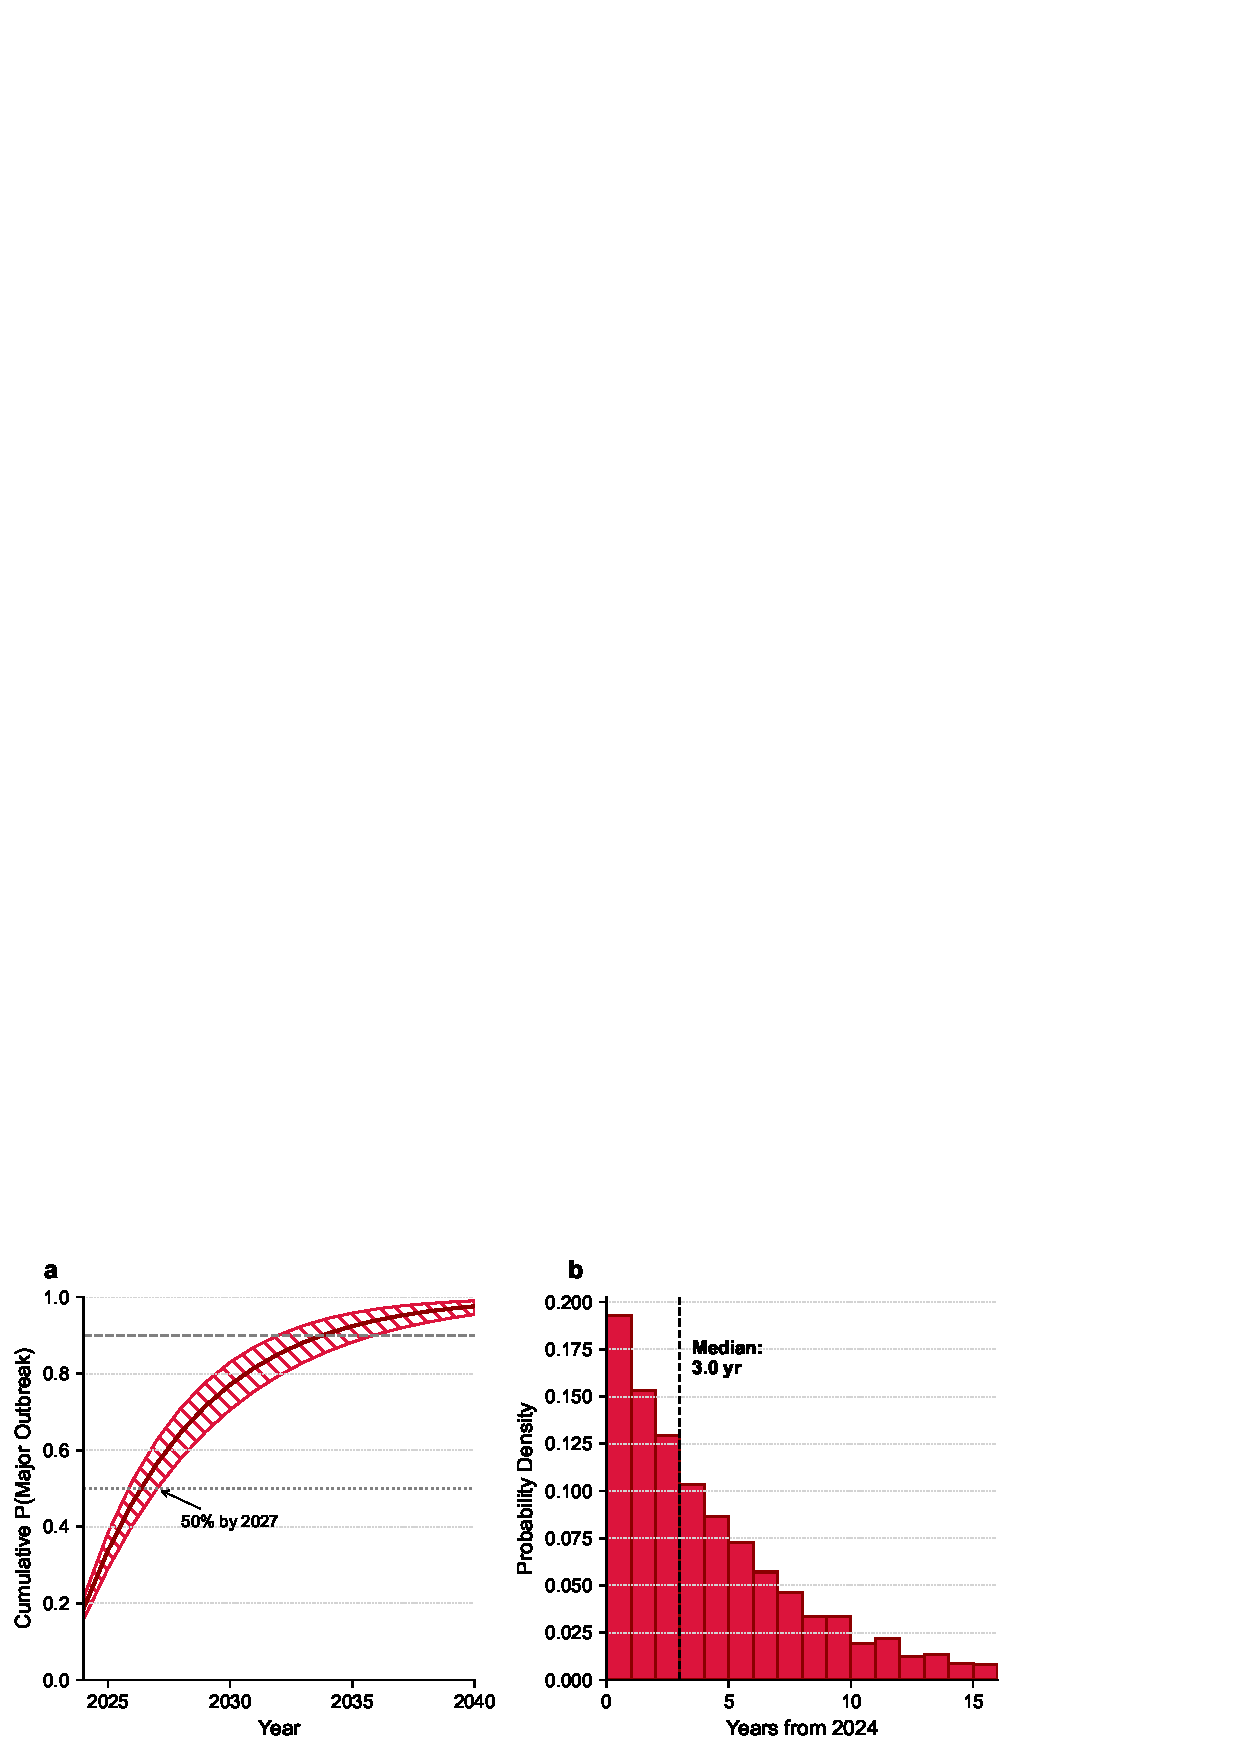
\includegraphics[width=\textwidth]{FigS2_OutbreakForecast.png}
\caption{\textbf{Supplementary Figure 2: Outbreak Probability Forecast.} Cumulative probability with 90\% CI. 50\% threshold crossed at year 4; 90\% threshold crossed at year 12.}
\label{fig:s2}
\end{figure}

\begin{figure}[ht]
\centering
\includegraphics[width=\textwidth]{FigS3_TornadoDiagram.png}
\caption{\textbf{Supplementary Figure 3: Tornado Diagram.} Most influential parameters: baseline outbreak probability ($\pm$49.8pp), critical network threshold ($\pm$17.8pp), methamphetamine multiplier ($\pm$16.6pp).}
\label{fig:s3}
\end{figure}

\begin{figure}[ht]
\centering
\includegraphics[width=\textwidth]{FigS4_ScenarioComparison.png}
\caption{\textbf{Supplementary Figure 4: Policy Scenario Comparison.} Current policy: 57\% 5-year risk, 4.5 years median. Full harm reduction: 41\% 5-year risk, 7.0 years median.}
\label{fig:s4}
\end{figure}

\begin{figure}[ht]
\centering
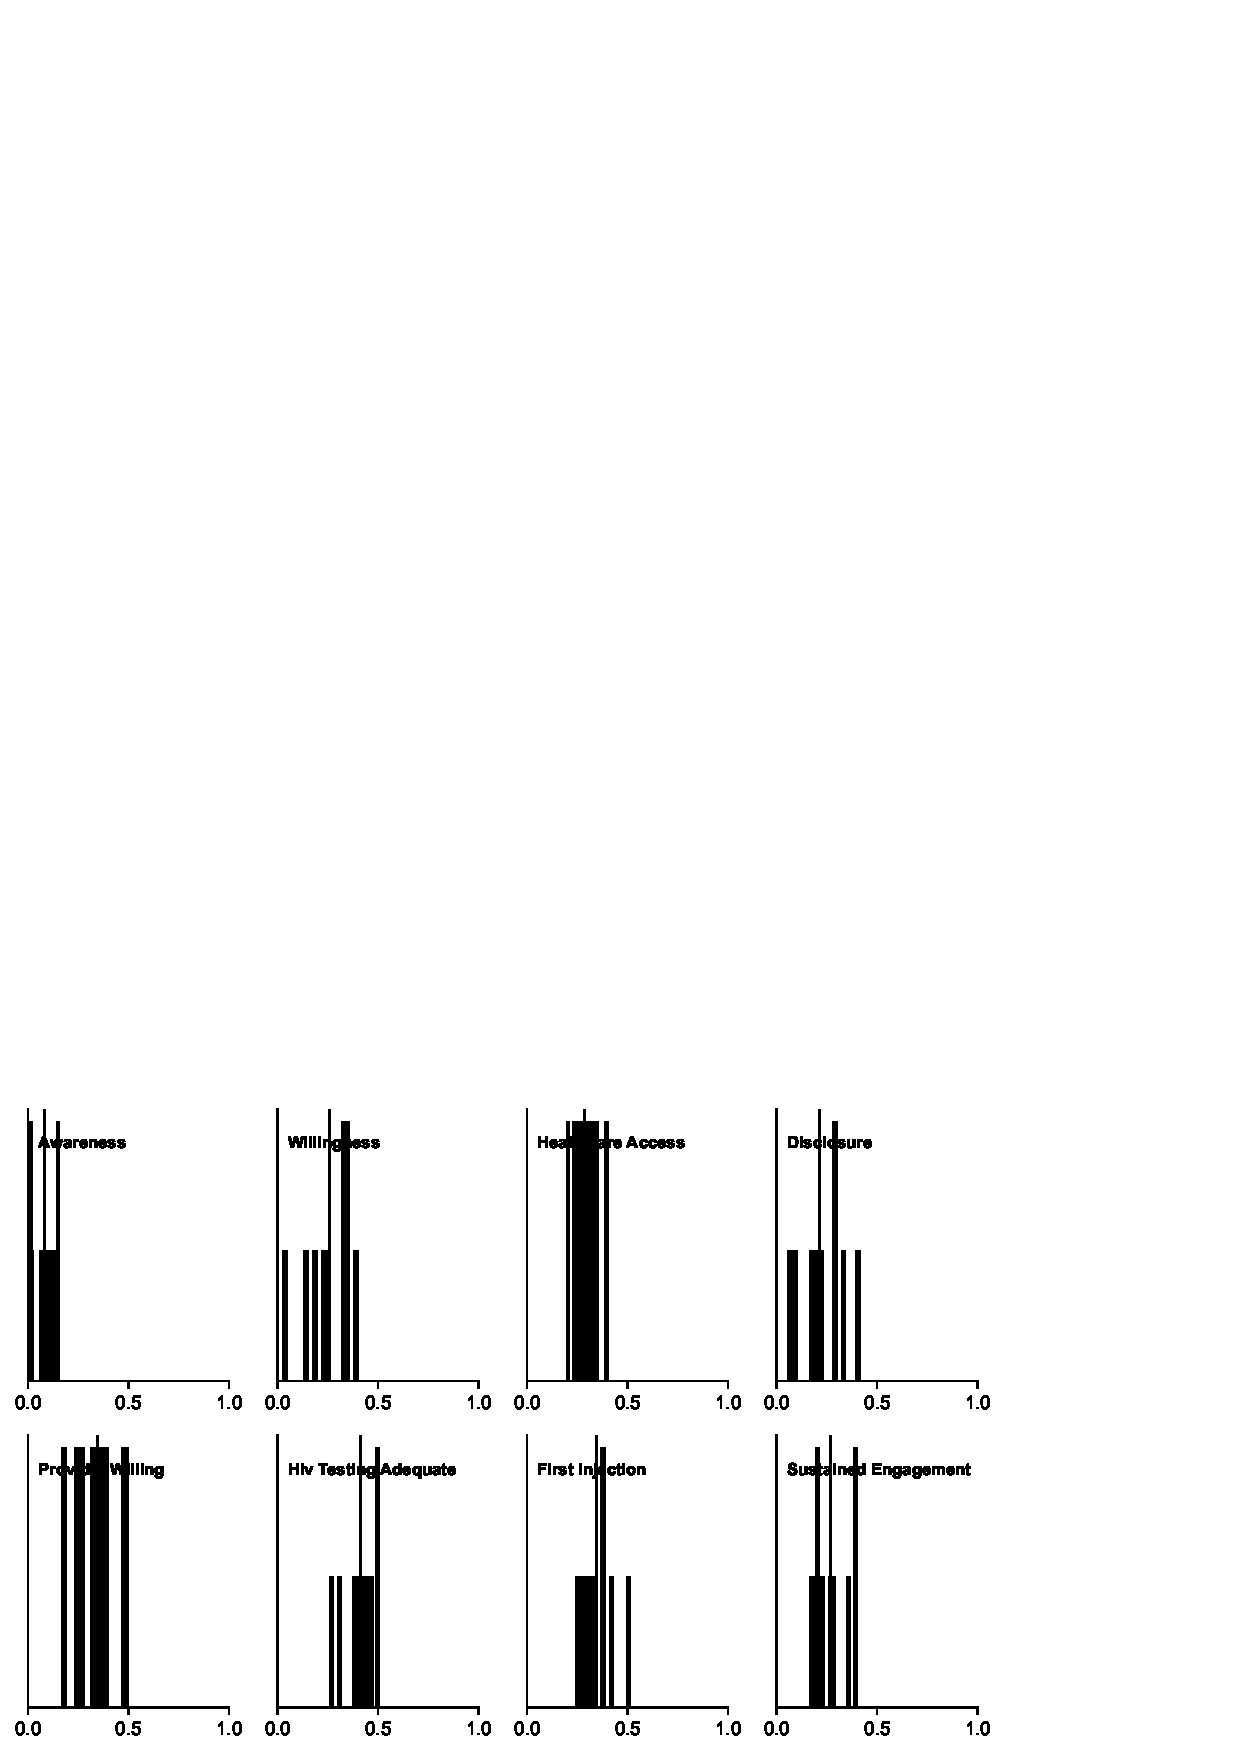
\includegraphics[width=\textwidth]{FigS5_CascadeUncertainty.png}
\caption{\textbf{Supplementary Figure 5: Cascade Uncertainty.} Probability distributions for each step under parameter uncertainty (n=1,000 PSA samples).}
\label{fig:s5}
\end{figure}

\begin{figure}[ht]
\centering
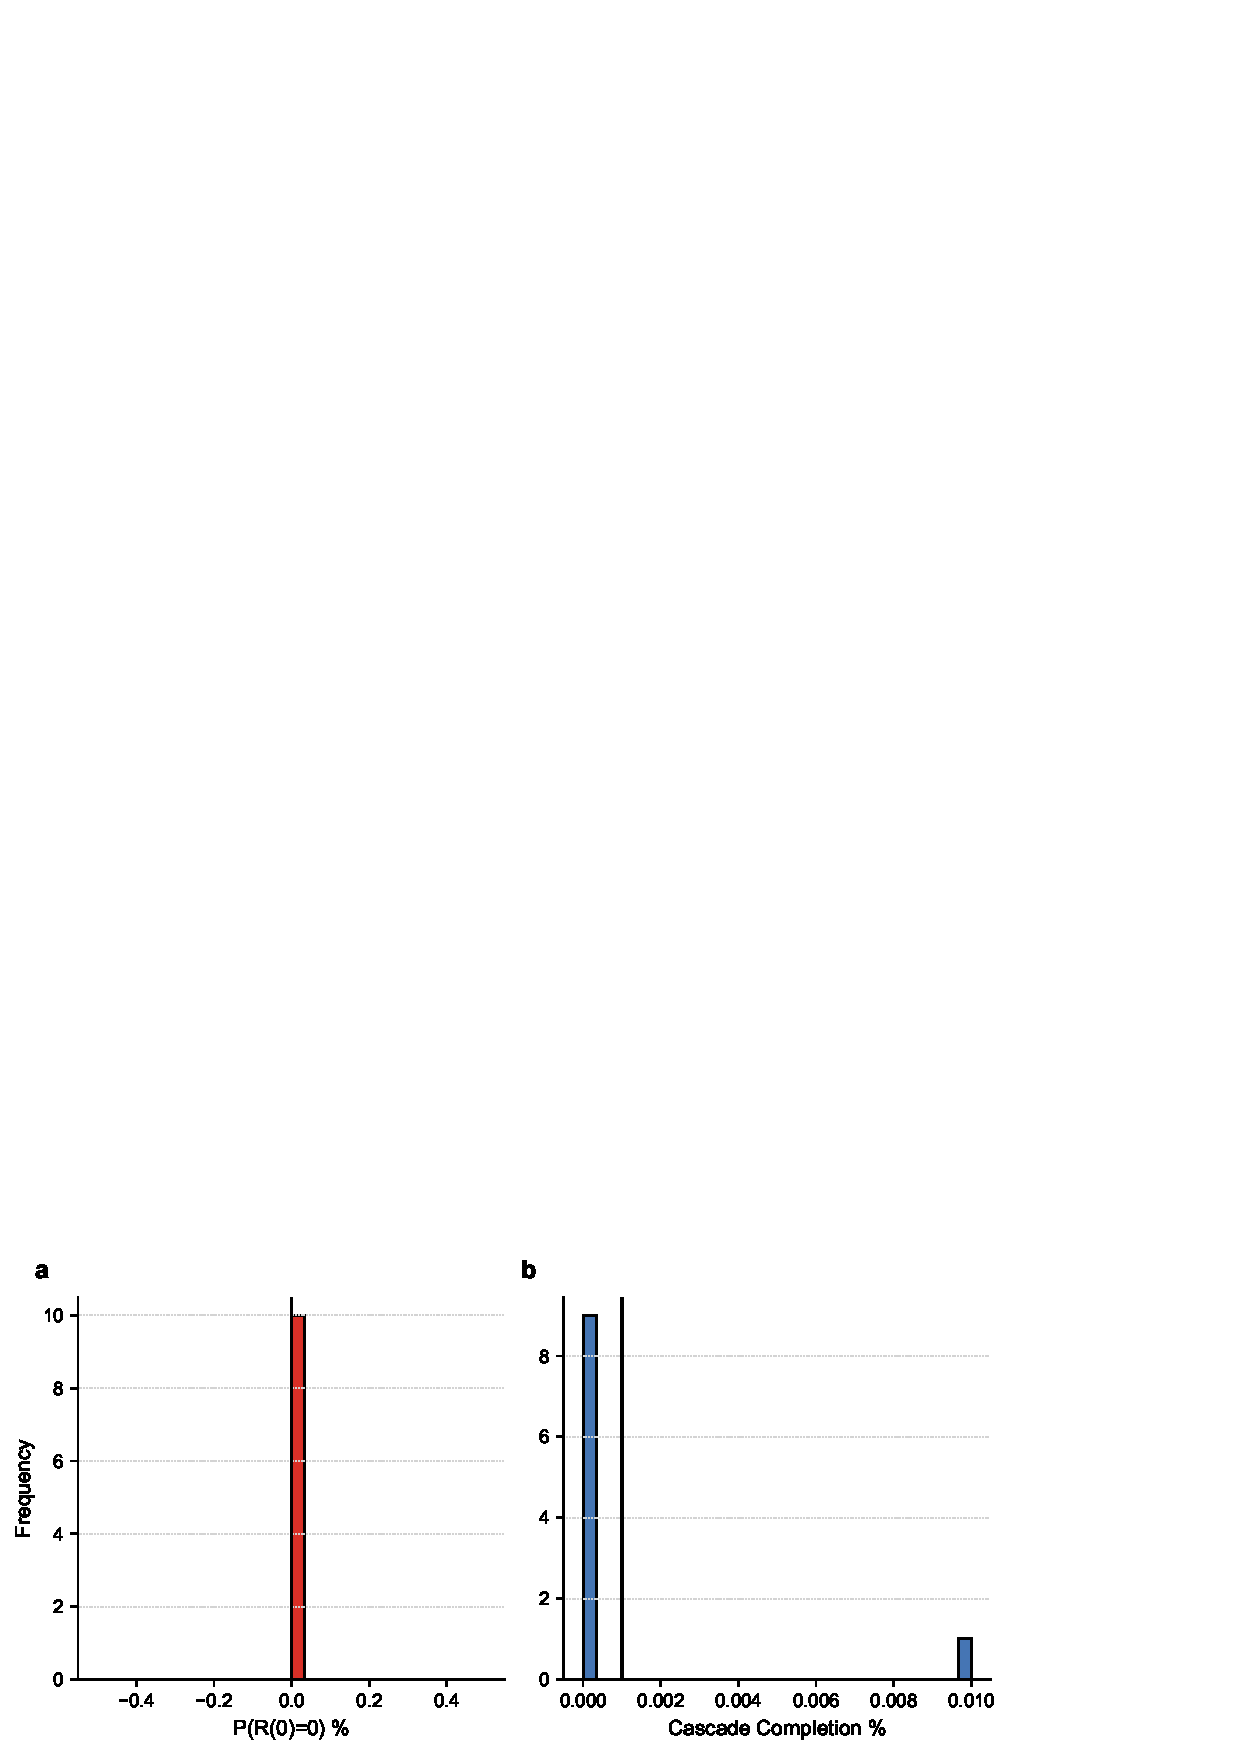
\includegraphics[width=\textwidth]{FigS6_R0ZeroDistribution.png}
\caption{\textbf{Supplementary Figure 6: P(\Rzero{}=0) Distribution.} Robustness demonstration: mean 0.0005\%, 90\% CI (0.00\%, 0.00\%) across 1,000 PSA samples.}
\label{fig:s6}
\end{figure}

\begin{figure}[ht]
\centering
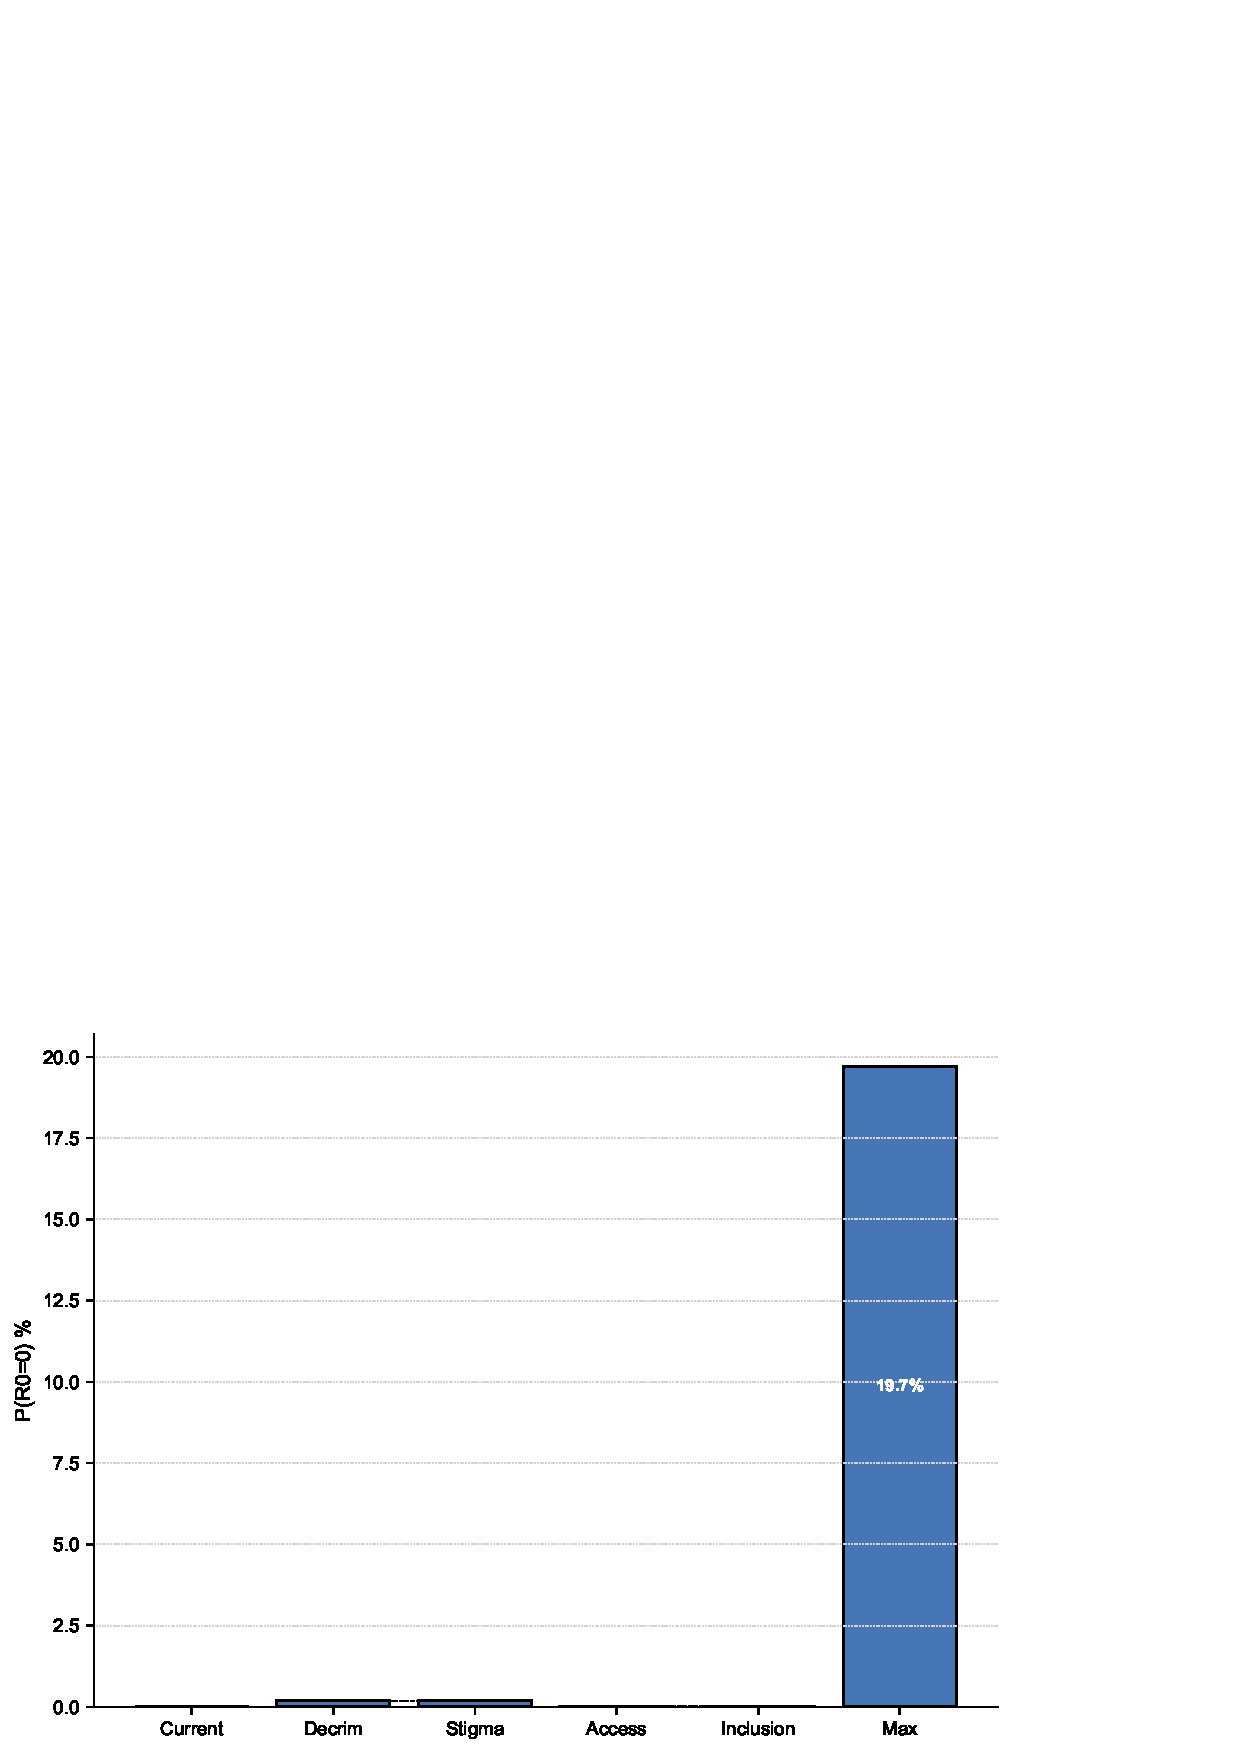
\includegraphics[width=\textwidth]{FigS7_BarrierRemoval.png}
\caption{\textbf{Supplementary Figure 7: Barrier Removal Waterfall.} Incremental effects: No criminalization (+0.23pp), No stigma (+0.01pp), Low-barrier access (+0.02pp), Full inclusion (+0.004pp), All removed (19.88\%).}
\label{fig:s7}
\end{figure}

\begin{figure}[ht]
\centering
\includegraphics[width=0.8\textwidth]{FigS8_StepImportance.png}
\caption{\textbf{Supplementary Figure 8: Step Importance.} No single step fix achieves epidemic control. Multiplicative cascade requires simultaneous intervention.}
\label{fig:s8}
\end{figure}

\newpage

% REFERENCES
\bibliographystyle{unsrtnat}
\bibliography{unified_MD}

\end{document}
